\documentclass[11pt, openany]{article}

\usepackage[T1]{fontenc}
\usepackage[utf8]{inputenc}
\usepackage[english, italian]{babel}
\usepackage{cancel}

\usepackage{hyperref}
\hypersetup{colorlinks=true,
	linkcolor=black,
	citecolor= black,
	filecolor=magenta,
	urlcolor=cyan,
}

\usepackage{geometry}
\geometry{
	a4paper,
	top=2.5cm,
	bottom=2cm,
	left=1.5cm,
	right=1.5cm,
	heightrounded,
	bindingoffset=5mm
}

\usepackage{amsmath}
\usepackage{amssymb}
\usepackage{amsthm}
\usepackage{tabularx}
\usepackage{booktabs}
\usepackage{caption}
\captionsetup{font = smaller}
\usepackage{enumitem}
\usepackage{blindtext}
\usepackage[x11names]{xcolor}
\usepackage{tcolorbox}
\usepackage{graphicx}
\usepackage{pdfpages}
\usepackage[export]{adjustbox}
\usepackage{cleveref}
\usepackage{multirow}
\usepackage{lipsum}



\theoremstyle{definition}
\newtheorem*{defn}{Definizione}
\newtheorem{exe}{Esercizio}[section]
\newtheorem{esem}{Esempio}[section]
\theoremstyle{plain}
\theoremstyle{remark}
\newtheorem*{warn}{ATTENZIONE}
\newtheorem*{svol}{Svolgimento}

\setcounter{secnumdepth}{-1}
\setcounter{tocdepth}{4}


\setlist[itemize]{nosep}
\usepackage{helvet}
\renewcommand{\familydefault}{\sfdefault}


\title{Relazione \\\textbf {Progetto A.A. 2022/2023 \\ ADAS made trivial: rappresentazione \underline{ispirata} alle
		interazioni in un sistema di guida autonoma}}
\author{Diciotti \hfill Matteo \\\\ 7072181 \and Manucci \hfill Agostino \\\\ 7084379 \and Montes Anacona \\ Àlvaro \\ 7117731}
\date{\today}

\begin{document}
	\maketitle
	\hrule
	\vspace{1cm}

	\part[Presentazione]{}
		\paragraph{Titolo}
			Progetto A.A. 2022/2023 – ADAS made trivial: rappresentazione \underline{ispirata} alle interazioni in un sistema di guida autonoma
		\paragraph{Autori}
			\footnotesize Lista degli autori ordinata per numero di matricola\\
			\normalsize
			\begin{tabularx}{\textwidth}[t]{p{4.5cm} p{3.5cm} p{2.5cm} r}
				\textbf{Matricola} 	& 	\textbf{Cognome} 	& 	\textbf{Nome} 	& \textbf{e-mail} 					\\\toprule
				7072181				&	Diciotti			&	Matteo			&	matteo.diciotti@stud.unifi.it	\\
				7084379				&	Mannucci			&	Agostino		&	agostino.mannucci@stud.unifi.it	\\
				7117731				&	Montes Anacona		&	Álvaro			&	alvaro.montes@stud.unifi.it
			\end{tabularx}

		\paragraph{Obiettivo}
			Obiettivo del progetto è costruire un’architettura, estremamente stilizzata e rivisitata, per sistemi ADAS, descrivendo possibili interazioni e alcuni comportamenti tra componenti in scenari specifici.

	\part{Introduzione}
		\paragraph{Introduzione al progetto}
			Un \textit{\textbf{A}dvanced \textbf{D}river \textbf{A}ssistance \textbf{S}ystem} è un sistema composto da varie componenti che cooperano affinché un veicolo o un mezzo possano assistere un conducente nella guida e, in alcuni contesti specifici e limitati, sostituirsi al guidatore stesso.\\
			Il progetto realizzato cerca di riprodurre il sistema simulativo di un ADAS presentato nella richiesta\footnote{Per visionare la richiesta dell'elaborato riferirsi al documento Allegato\_1.pdf compreso nella cartella del progetto} dell'elaborato nella quale sono definite varie componenti suddivise in quattro gruppi: \textit{interfaccia}, \textit{attuatori}, \textit{sensori} e \textit{controllo}.\\
			La simulazione è resa effettiva dall'inserimento di stringhe rappresentanti le azioni che dovrebbero essere eseguite dalle varie componenti di un ADAS in dei file di log specifici per ogni componente ed in un terminale adibito alla visualizzazione dei comandi inviati da parte dell'unità di controllo. In particolare le componenti implementate sono nove, sette obbligatorie e due facoltative\footnote{Per conoscere quali elementi facoltativi sono stati implementati visionare la tabella a pagina~\pageref{tab:facoltativi}}.\\
			I \underline{sensori}, attraverso l'acquisizione di dati dal file \textit{urandomARTIFICIALE.binary} o dal dispositivo \textit{/dev/uran-dom}, utilizzato come sorgente binaria casuale, simulano l'acquisizione di dati da parte di sensori reali e li inviano all'unica componente di controllo, la componente \textit{central-ECU}.
			Gli \underline{attuatori}, invece, ricevono messaggi dall'unità di controllo ed eseguono scritture negli appositi file di log, simulando così l'azione di un attuatore reale.
			Infine, la componente con cui si interfaccia l'esecutore del programma è la \underline{Human-Machine Interface} che simula l'interfaccia del guidatore attendendo da parte dallo stesso utente alcuni specifici comandi(in questo caso scritti su di un emulatore di terminale) e mostrando le conseguenze di questi ed alcuni risultati: nel contesto della simulazione saranno mostrati su di un secondo emulatore di terminale tutti i comandi che l'unita di controllo ha inviato alle varie componenti del sistema.

		\paragraph{Impostazione del lavoro}
			Al fine di realizzare un sistema che simulasse un ADAS sono state eseguite alcune fasi per il completamento del programma: l'analisi delle richieste, la strutturazione teorica dell'architettura del sistema, l'implementazione pratica, la verifica e revisione dell'elaborato.\\
			Ad una prima fase di studio delle richieste congiunta tra gli autori del progetto è immediatamente succeduta la fase di strutturazione dello stesso, anch'essa svolta unitamente tra i relatori, giungendo alla teorizzazione dell'architettura mostrata in figura~\ref{fig:gerarchia}. Sono stati quindi divisi i lavori per l'implementazione del programma tra i componenti del gruppo e uniti gli elaborati in un unico componimento comprensivo di makefile e file binari per l'esecuzione in modalità \textit{ARTIFICIALE} del programma. Sono state quindi eseguite ciclicamente le due fasi di verifica e di modifica: nella prima fase sono stati svolti test per verificare il corretto funzionamento dell'elaborato in entrambe le modalità e nella seconda fase sono state apportate le modifiche necessarie affinché il programma producesse i risultati attesi. Infine e` stata prodotta la presente relazione.
	\part{Specifiche}
		\paragraph{Caratteristiche HW e SW}
		Per l'implementazione sono stati utilizzati tre hardware differenti con tre sistemi operativi differenti:
		\begin{itemize}
			\item \textbf{ArchLinux}, architettura x86\_64, kernel Linux 6.1.34-1-LTS
			\item \textbf{Manjaro 23.0.0}, architettura x86\_64, kernel Linux 5.15.114-2-MANJARO
			\item \textbf{Ubuntu 20.04}, architettura x86\_64, kernel Linux 5.15.0-75-generic
		\end{itemize}
		Il progetto è stato ideato avendo come obbiettivo un programma portatile\footnote{NOTA SULLA PORTABILITÀ: è stato preso come riferimento per la portabilità del sistema lo standard \textbf{\_POSIX\_C\_SOURCE 200809L}, il quale garantisce un'ottimo grado si portabilita su sistemi \textit{UNIX} e \textit{UNIX-like}. È altresì necessario notare però che l'utilizzo di alcune funzioni e system-callS, come signal(2) la quale è sconsigliata dai manuali \textit{POSIX} per questioni di portabilità, e l'utilizzo della sorgente /dev/urandom potrebbero limitare lo spettro di piattaforme  su cui eseguire il programma ai ``soli'' sistemi \textit{UNIX-like}. Dato il contesto accademico, è stato comunque preferito l'utilizzo delle funzioni suddette per non discostarsi eccessivamente degli argomenti del corso.} che fosse preimpostato per eseguire su di un sistema \textbf{\underline{Ubuntu Linux 22.04}}.
		\paragraph{Istruzioni compilazione ed esecuzione}
			Nel presente paragrafo si mostrano i passaggi necessari affinché si possa eseguire il programma sul proprio dispositivo:
			\subparagraph{Estrazione e compilazione}
				\begin{enumerate}
					\item Estrarre il file .zip in una cartella a piacimento. (Esempi comando: \texttt{tar~-x~\$PROJECT\_NAME\$; \texttt{7z~x~\$PROJECT\_NAME\$}});
					\item Spostarsi nella cartella creatasi con l'estrazione. (Esempio comando: \texttt{cd~./\$PROJECT\_NAME\_FOLDER\$});
					\item Eseguire i comandi di compilazione e  installazione del programma: \texttt{make; make install}
				\end{enumerate}
				Terminata questa procedura il programma dovrebbe risultare pronto per l'esecuzione.
				\subparagraph{Esecuzione}
					\begin{enumerate}
						\item Assicurarsi di essere con un terminale nella directory sorgente del programma, la stessa contenente le cartelle bin, src, include etc. e il file eseguibile \textit{ADAS-simulator}.
						\item Avviare l'inizializzazione e l'esecuzione del programma tramite la chiamata di \texttt{./ADAS-simulator \$MODALITÀ\$}, dove \texttt{\$MODALITÀ\$} rappresenta la modalità \texttt{ARTIFICIALE} o \texttt{NORMALE} del programma\footnote{Per la comprensione delle differenze delle modalita di esecuzione riferirsi al paragrafo 4 della richiesta \textit{Allegato\_01.pdf}}.
						Oltre al secondo argomento (il quale risulta obbligatorio, pena la mancata esecuzione del programma e la restituzione di un errore di sintassi), il comando supporta anche l'opzione \texttt{$--$term} nella quale si può specificare l'emulatore di terminale che si desidera utilizzare come terminale di output. L'emulatore impostato di default è \textit{gnome-teminal}. Per utilizzarne uno differente inserire il comando di shell che apre un nuovo terminale tipologia scelta (Esempio: \texttt{./ADAS-simulator ARTIFICIALE --term konsole} o \texttt{./ADAS-simulator ARTIFICIALE --term xfce4-terminal})
						\item Eseguito il comando dovrebbe aprirsi automaticamente un nuovo terminale rappresentante il terminale di output. Non eseguire alcun comando sul terminale di output e posizionarsi con il cursore sul terminale di input, ovvero il terminale nel quale è stato eseguito il comando di avvio del programma.
						\item Il programma è inizializzato: si possono ora eseguire i comandi INIZIO, PARCHEGGIO per iniziare l'esecuzione del programma e successivamente ARRESTO per simulare un arresto del veicolo\footnote{Per la comprensione dei comandi inseribili dal terminale rifarsi al paragrafo 2, sotto-paragrafo \textit{Human-Machine Interface}, della richiesta \textit{Allegato\_01.pdf}}.
				\end{enumerate}

				\begin{figure}[b!]
					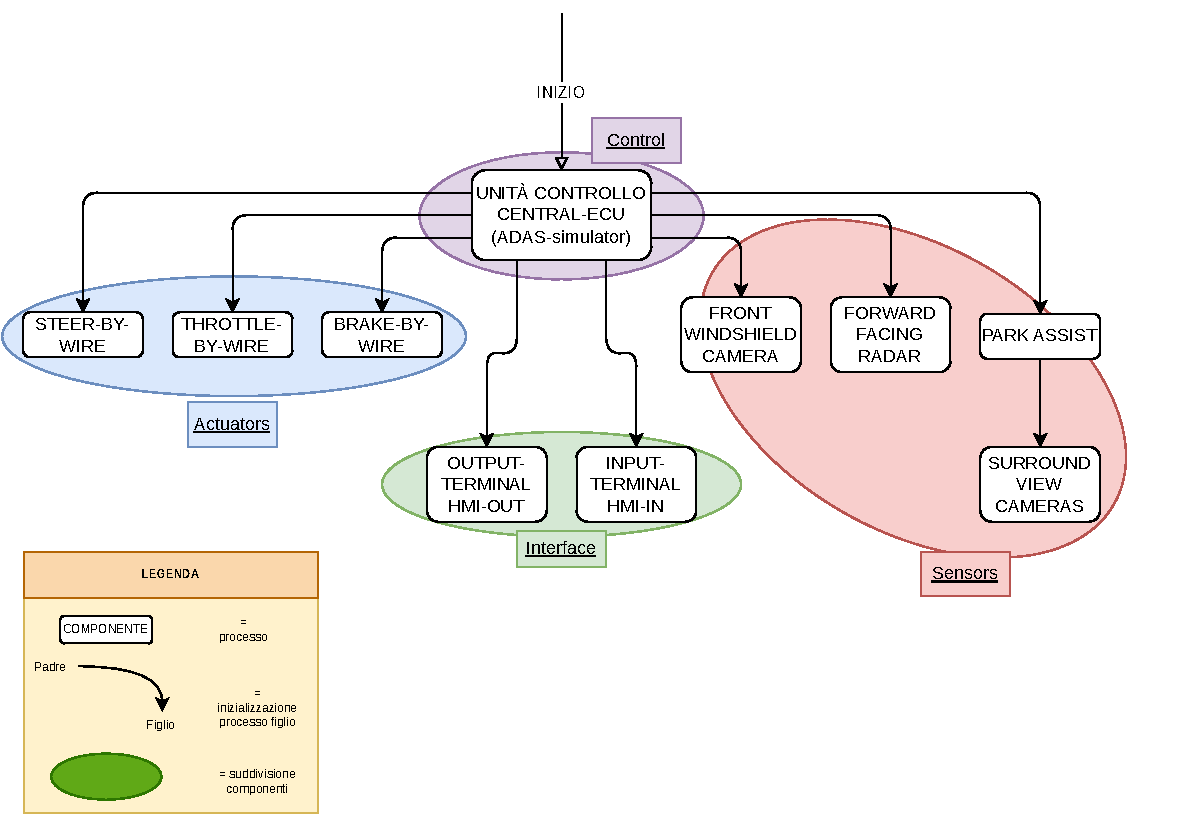
\includegraphics[scale=0.7, center]{./include/SO_Progetto_Diagrammi-Gerarchia.pdf}
					\caption{In figura è mostrata la gerarchia implementata nel programma. La \textit{central-ECU} rappresenta il processo antenato di tutte gli altri processi, \textit{park assist} risulta genitore dei \textit{surround view cameras}.}
					\label{fig:gerarchia}
				\end{figure}
		\paragraph{Elementi facoltativi}
			La tabella a pagina~\pageref{tab:facoltativi} mostra gli elementi facoltativi implementati seguiti da una breve descrizione dell'implementazione.
			\begin{tcolorbox}[width=\textwidth,move upwards= -16pt , colback={Cornsilk2}]
				\begin{tabularx}{\textwidth}{lXcX}
					\textbf{\#}	&	\textbf{Elemento facoltativo}	&	\textbf{Realizzato (SI/NO)}	&	\textbf{Descrizione dell'implementazione con indicazione del metodo/i principale/i} \\\toprule\vspace{.1cm}
					1	&	Ad ogni accelerazione, c’è una probabilità di $10^{-5}$ che l’acceleratore fallisca. In tal caso, il componente \textit{throttle control} invia un \underline{segnale} alla \textit{central-ECU} per evidenziare tale evento, e la central-ECU avvia la procedura di \textit{ARRESTO} & SI	&
					Metodo: \textit{throttle-control} $\rightarrow$ \textit{throttle\_failed()}. Il metodo, tramite la funzione \texttt{rand()} della \texttt{libc} ottiene un numero aleatorio il cui modulo per 10000 simula una probabilità del 1 su $10^5$ se eguagliato a 0\footnote{La probabilità non risulta esattamente $10^{-5}$ dato l'intervallo di valori producibili da \texttt{rand()}, ma la differenza risulta trascurabile ai fini del progetto.} \\\vspace{0.1cm}
					2	&	Componente \textit{forward facing radar}	&	SI	&
					Sorgente \textit{bytes-sensors.c}. Il processo esegue un ciclo infinito di letture, invii e scritture su file di log.\\\vspace{0.2cm}
					3	&	Quando si attiva l’interazione con park assist, la \textit{central-ECU} sospende (o rimuove) tutti i sensori e attuatori, tranne \textit{park assist} e \textit{surround view cameras}	&	SI	&
					Nella \textit{central-ECU} vengono segnalati con un \texttt{SIGKILL} tutti i processi attuatori e sensori esistenti prima di procedere all'inizializzazione del parcheggio.\\\vspace{0.1cm}
					4	&	Il componente \textit{park assist} non è generato all'avvio del sistema, ma creato dalla \textit{central-ECU} al bisogno	&	SI	&
					La \textit{central-ECU} esegue la \texttt{fork} per la creazione di \textit{park-assist} in \textit{park\_assist\_init()}, il quale inizializza il processo prima di entrare nel ciclo di parcheggio.\\\vspace{0.1cm}
					5	&	Se il componente \textit{surround view cameras} è implementato, \textit{park assist} trasmette a \textit{central-ECU} anche i byte ricevuti da \textit{surround view cameras}	&	SI	&
					Nel ciclo principale di \textit{park-assit} si esegue una \texttt{read} da \textit{cameras.pipe} (non bloccante) e una \texttt{write} dei dati ricevuti sulla socket \textit{assist.sock} \\\vspace{0.1cm}
					6	&	Componente \textit{surround view cameras}	&	SI	&
					Sorgente \textit{bytes-sensors.c}. Vedi facoltativo 2 - \textit{forward facing radar}	\\\vspace{0.1cm}
					7	&	Il comando di \textit{PARCHEGGIO} potrebbe arrivare mentre i vari attuatori stanno eseguendo ulteriori comandi (accelerare o sterzare). I vari attuatori interrompono le loro azioni, per avviare le procedure di parcheggio	&	SI	&
					Nella \textit{central-ECU}, nel ciclo principale, dopo la lettura da hmi-input, \textit{kill(-processes\_groups.actuators\_gro-up, SIGKILL)}. Si esegue la segnalazione di chiusura immediata dei processi  \textit{steer} e \textit{throttle} (brake rimane per il ciclo di frenata).\\
					8	&	Se la \textit{central-ECU }riceve il segnale di fallimento accelerazione da \textit{throttle control}, imposta la velocità a 0 e invia all'output della \textit{HMI} un messaggio di totale terminazione dell'esecuzione	&	SI	&
					Nella \textit{central-ECU}, una volta ricevuto il segnale di \textit{PERICOLO}, gestito tramite \textit{ECU\_signal\_handler} si esegue la procedura di arresto, stampa la stringa di terminazione e si conclude l'esecuzione dei processi.

				\end{tabularx}
				\label{tab:facoltativi}
			\end{tcolorbox}
	\part{Descrizione architettura sistema}
		Nella seguente sezione viene presentata l'architettura del progetto e le scelte implementative prese, cercando di descrivere i motivi che hanno portato alle singole decisioni prese.

		\paragraph{Implementazione componenti}
			\footnotesize Segue una tabella nella quale si mostrano quali sorgenti implementano le componenti
			\normalsize

			\begin{tcolorbox}[width=\textwidth,colback={Cornsilk2}]\label{tab:sorgenti}
				\begin{tabularx}{\textwidth}{p{8cm}  l}
					\textbf{Componente}			&	\textbf{Sorgente}	\\\toprule
					Human-Machine Interface 	& 	hmi-input.c			\\
												&	hmi-output.c		\\\midrule
					steer-by-wire				&	steer-by-wire.c		\\\midrule
					throttle control			&	throttle-control.c	\\\midrule
					brake-by-wire				&	brake-by-wire.c		\\\midrule
					front windshield camera		&	windshield-camera.c	\\\midrule
					forward facing radar		&	bytes-sensors.c		\\\midrule
					park assist					&	park-assist.c		\\\midrule
					surround view cameras		&	bytes-sensors.c		\\\midrule
					central-ECU					&	central-ECU.c
				\end{tabularx}
			\end{tcolorbox}

		\paragraph{Gerarchia del programma}
			La gerarchia del progetto è stata ottenuta dalla richiesta cercando di massimizzare la semplicità.
			Questa rappresenta lo scheletro del progetto e definisce quindi il flusso di lavoro dello stesso. In particolare si può notare in figura~\ref{fig:gerarchia} che esistono due soli processi che inizializzano dei figli, ovvero l'unita di controllo centrale \textit{central-ECU}, che rappresenta anche il programma genitore di tutto il sistema, e \textit{park-assist}, che inizializza il suo unico figlio \textit{surround-view cameras}.\\
			È stato scelto di rendere l'unità di controllo la componente genitore di tutto il sistema dato che è in collegamento con la quasi totalità dei processi agenti, cosicché il sistema fosse inizializzato e gestito nel flusso di questa. La soluzione sembrava essere coerente con la strutturazione dei sistemi ADAS reali.\\
			Nella \textit{central-ECU} vengono quindi inizializzati le pipe, vengono eseguite varie \texttt{fork} per la creazione e la connessione in lettura/scrittura ai pipe degli attuatori, delle due componenti relative alla \textit{Human-Machine Interface} ed infine i due sensori \textit{front windshield camera} e \textit{forward facing radar}. L'unico componente figlio della \textit{central-ECU} non immediatamente inizializzato rimane \textit{park-assist}\footnote{La decisione di non inizializzare il componente immediatamente deriva dalla richiesta, ovvero dall'elemento facoltativo numero 4. Vedi la tabella di pagina~\pageref{tab:facoltativi}.} il quale verrà inizializzato (comprensivo della socket che utilizzerà per comunicare con la \textit{central-ECU}) e messo in esecuzione dalla stessa unità di controllo quando questa riceverà un comando di \textit{PARCHEGGIO} dall'interfaccia oppure dal sensore \textit{windshield camera}.\\
			Con le stesse motivazioni è stato deciso di rendere la \textit{central-ECU} "server" nella connessione socket tra questa e \textit{park assist}. In questo modo sarà sempre la central-ECU a gestire il flusso di lavoro e a dettare i tempi del sistema.
			All'avvio della procedura di parcheggio, successivamente al ciclo di rallentamento, la \textit{central-ECU} avvierà la componente \textit{park-assist}, la quale si connetterà alla socket e inizializzerà \textit{surround-view cameras}. Terminata l'inizializzazione, l'unita di controllo invierà un messaggio (``INIZIO'') tramite la socket a \textit{park assist}, la quale leggerà per 30 iterazioni (intervallate da \texttt{sleep(1)}) i dati dalla sorgente binaria e i dati ricevuti dalla componente figlia tramite la pipe di comunicazione e li invierà alla \textit{central-ECU} che li scandirà alla ricerca di particolari pattern\footnote{Per conoscere i pattern binari (espressi in codifica esadecimale) prendere visione del paragrafo 2, sotto-paragrafo \textit{Componente central-ECU} della richiesta \textit{Allegato\_01.pdf}}. Se non venissero evidenziate congruenze allora la central-ECU informerà tramite un messaggio (``CONTINUA'') \textit{park assist} perché possa proseguire nell'iterazione successiva. Se così non fosse allora verrà posto sulla socket un messaggio di riavvio (``RIAVVIO''), affinché il parcheggio inizi nuovamente il ciclo delle 30 iterazioni. Concluse le 30 iterazioni senza ''insuccessi'' allora l'esecuzione del parcheggio risulterà conclusa e il processo terminerà.

		\paragraph{IPC nel sistema}
			In figura~\ref{fig:comunicazione}, a pagina~\pageref{fig:comunicazione}, si mostra una schematizzazione molto stilizzata della rete comunicativa del sistema.
			La struttura di comunicazione maggiormente sfruttata all'interno del sistema è la \textbf{pipe} la quale implementa 8 canali di comunicazione su 9 (segnali esclusi). Il motivo della scelta delle \textbf{pipe} a discapito di altri metodi risiede nel fatto che le comunicazioni sono sostanzialmente unidirezionali (sensori $\rightarrow$ unità di controllo, unità di controllo $\rightarrow$ attuatori, con le due evidenti eccezioni di \textit{park assist} e di \textit{surround-view cameras}). La scelta ha permesso di implementare un sistema relativamente semplice, con un'unica \textbf{socket}, struttura più complessa da implementare..\\
			Il protocollo di gestione dei canali risulta unico per tutte le tipologie di canali e per tutti i processi: il processo padre, l'unico processo che comunica con i propri processi figli, produce ed inizializza correttamente il file \texttt{.pipe} o \texttt{.sock} (rappresentante socket \texttt{UNIX}) nella directory \textit{tmp} (dopo aver avuto l'accortezza di eliminare creazioni pendenti da vecchie esecuzioni tramite un \texttt{unlink}), il processo figlio si connette con  l'adeguata procedura, differente tra pipe e socket, al canale di comunicazione nella fase inizializzazione del processo. Se la connessione non dovesse riuscire (se la \texttt{openaT} o la \texttt{connect} dovessero generare un errore) il figlio terminerebbe con codice di errore \texttt{EXIT\_FAILURE} e stamperebbe il codice tramite \texttt{perror(3)} nel file di log adibito a \textit{stderr}: \texttt{./log/errors.log}\\
			Per l'implementazione del parcheggio il canale di comunicazione è stato strutturato sotto forma di una socket per semplificare la comunicazione tra i due processi e perché la gestione del contenuto della socket fosse meno soggetto a problemi di concorrenza. Ogni volta che la \textit{central-ECU} riceve dalla socket uno dei pattern non ammissibili, che simulano una situazione di parcheggio non accettabile, il protocollo prevede che invii un messaggio di riavvio a \textit{park assist}. Il protocollo prevede che ad ogni ciclo \textit{park assist} legga dalla pipe non bloccante \textit{cameras.pipe} i byte da inviare alla \textit{central-ECU} e che li inoltri. Se, eseguito l'invio, riceve dalla \textit{central-ECU} un messaggio che indica la necessità di riavvio, allora non fa altro che resettare il contatore di iterazioni e riprendere il ciclo.
			\begin{figure}[t]
				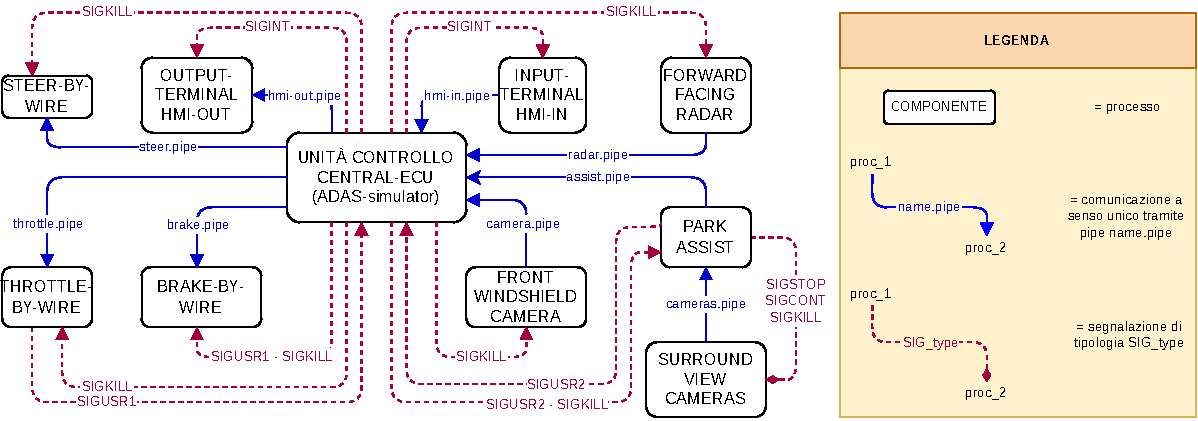
\includegraphics[scale=0.9, center]{./include/SO_Progetto_Diagrammi-Comunicazione.pdf}
				\caption{In figura sono rappresentati i percorsi comunicativi inseriti nel sistema: sono presenti 8 pipe, 1 socket e 12 di segnalazioni, 5 rappresentate e 7 assenti. Sono infatti stati esclusi i percorsi delle segnalazioni \texttt{SIGKILL} per alleggerire il grafico.}
				\label{fig:comunicazione}
			\end{figure}
			\normalsize
		\paragraph{Gestione dei log}
			I log rappresentano, nel sistema implementato, la simulazione delle componenti reali, ovvero mostrano le azioni agite dalle varie componenti.\\
			Per ogni componente, esclusa la \textit{Human-Machine Interface}, è presente un file di log specifico nel quale vengono scritte le azioni eseguite.
			Gli inserimenti nel file di log seguono le richieste specificate nella richiesta del progetto \textit{Allegato\_1.pdf}.
			Perché le shell di input e di output risultassero pulite da ogni eventuale segnalazione diretta allo \textit{stderr} è stato adottato il file \texttt{./log/errors.log} come soluzione per inserirvi tutti i messaggi dirette a questo.

		\paragraph{Funzioni condivise}
			Durante lo sviluppo del sistema sono risultate utili la creazione di alcune strutture, come ad esempio \texttt{struct process}, la definizione di alcune funzioni di utilità generale per il sistema e di alcune macros, anch'esse sfruttate in più contesti. Tutto ciò è stato inserito all'interno del sorgente \texttt{service-functions.c}, il cui header risulta quindi \texttt{service-functions.h}.

	\part{Esempi di esecuzione}
		Nella seguente sezione sono mostrati 2 esempi di funzionamento: il primo mostra un funzionamento in modalità ARTIFICIALE con comando dato da input ``INIZIO'' e alcuni ``ARRESTO'', nel secondo si esegue in modalità NORMALE direttamente il parcheggio con un terminale selezionato. All'interno dello \texttt{.zip} è stata  inserita una cartella \textit{Esempi di funzionamento} nella quale sono stati inseriti i file di log risultanti dalle esecuzioni presentate.
		\paragraph{Esempio: ARTIFICIALE standard}
			Il presente esempio è teso a mostrare un'esecuzione tipica del programma.
			Il programma è stato eseguito tramite il comando \texttt{./ADAS-simulator ARTIFICIALE}. Non appena il programma si è inizializzato è stato inserito il comando ``INIZIO''. Il programma si è avviato correttamente iniziando ad inserire sul terminale di output i comandi impartiti da parte della \textit{central-ECU} alle rispettive componenti. Sono stati inseriti, durante l'esecuzione, quattro comandi di ``ARRESTO''. Il programma ha eseguito correttamente la procedura di arresto, bloccando istantaneamente l'auto e ripartendo la corsa istantaneamente. La procedura di parcheggio, ultimo comando da parte della \textit{windshield camera}, è terminata dopo 30 iterazioni (30 secondi).

		\paragraph{Esempio: NORMALE terminale personalizzato}
			Il presente esempio è teso a mostrare un'esecuzione del programma relativamente atipica e potenzialmente problematica, un'esecuzione nella quale l'utente inserisce inizialmente una stringa non accettabile, poi il comando ``ARRESTO'', sebbene il mezzo non sia ancora in movimento ed infine il comando ``PARCHEGGIO''.
			Il programma è stato eseguito tramite il comando \texttt{./ADAS-simulator NORMALE --term xfce4-terminal}. Non appena il programma si è inizializzato è stato inserita come comando ``42'', che è risultata non accettabile, poi ``ARRESTO'', anch'essa non accettabile, ed infine ``parcheggio'' che ha dato il via alla procedura di parcheggio, terminata con successo dopo un ciclo di iterazioni. È stata infatti implementata una funzione per il confronto tra stringhe case-insensitive per i comandi dalla hmi-input.

	\newpage
	\hrule
	\tableofcontents

\end{document}